\documentclass[letterpaper, twoside]{article}

\usepackage{blindtext} % Package to generate dummy text throughout this template 

\usepackage[sc]{mathpazo} % Use the Palatino font
\usepackage[T1]{fontenc} % Use 8-bit encoding that has 256 glyphs
\linespread{1.05} % Line spacing - Palatino needs more space between lines
\usepackage{microtype} % Slightly tweak font spacing for aesthetics

\usepackage[english]{babel} % Language hyphenation and typographical rules

\usepackage[hmarginratio=1:1,top=32mm,columnsep=20pt]{geometry} % Document margins
\usepackage[hang, small,labelfont=bf,up,textfont=it,up]{caption} % Custom captions under/above floats in tables or figures
\usepackage{booktabs} % Horizontal rules in tables

\usepackage{lettrine} % The lettrine is the first enlarged letter at the beginning of the text

\usepackage{enumitem} % Customized lists
\setlist[itemize]{noitemsep} % Make itemize lists more compact

\usepackage{abstract} % Allows abstract customization
\renewcommand{\abstractnamefont}{\normalfont\bfseries} % Set the "Abstract" text to bold
\renewcommand{\abstracttextfont}{\normalfont\small\itshape} % Set the abstract itself to small italic text

\usepackage{titlesec} % Allows customization of titles
\renewcommand\thesection{\Roman{section}} % Roman numerals for the sections
\renewcommand\thesubsection{\roman{subsection}} % roman numerals for subsections
\titleformat{\section}[block]{\large\scshape\centering}{\thesection.}{1em}{} % Change the look of the section titles
\titleformat{\subsection}[block]{\large}{\thesubsection.}{1em}{} % Change the look of the section titles

\usepackage{fancyhdr} % Headers and footers
\pagestyle{fancy} % All pages have headers and footers
\fancyhead{} % Blank out the default header
\fancyfoot{} % Blank out the default footer
\fancyhead[C]{Variational generation of images by deep spatial architectures $\bullet$ June 2017 } % Custom header text
\fancyfoot[RO,LE]{\thepage} % Custom footer text

\usepackage{titling} % Customizing the title section
\usepackage{hyperref} % For hyperlinks in the PDF
\usepackage{amsmath}
\usepackage{tikz}
\usepackage{multicol}
\usepackage{float}
\usetikzlibrary{fit,positioning}

%----------------------------------------------------------------------------------------
%   TITLE SECTION
%----------------------------------------------------------------------------------------

\setlength{\droptitle}{-4\baselineskip} % Move the title up

\pretitle{\begin{center}\Huge\bfseries} % Article title formatting
\posttitle{\end{center}} % Article title closing formatting
\title{Variational generation of images by deep spatial architectures} % Article title
\author{%
\textsc{Arthur Viv\'e} \\% \thanks{A thank you or further information} \\[1ex] % Your name
Advisor: Yali Amit \\
Department of Statistics\\
University of Chicago \\ % Your institution
%\normalsize \href{mailto:john@smith.com}{john@smith.com} % Your email address
%\and % Uncomment if 2 authors are required, duplicate these 4 lines if more
%\textsc{Jane Smith}\thanks{Corresponding author} \\[1ex] % Second author's name
%\normalsize University of Utah \\ % Second author's institution
%\normalsize \href{mailto:jane@smith.com}{jane@smith.com} % Second author's email address
}
\date{\today} % Leave empty to omit a date
\renewcommand{\maketitlehookd}{%
\begin{abstract}
\noindent Given the recent successes of neural networks at generating images, we make an attempt to augment those models with high level information. More precisely, by introducing equivariance to a broad set of spatial transformation into the variational autoencoder \cite{Kingma.aevb}, we manage to better model natural images, leveraging the power of neural networks while staying in the statistical framework of variational inference. Such models allow us to sample credible candidates directly from the image distribution. Our models are based on dense neural networks and spatial transformer layers \cite{Jaderberg.stn}. We will show that by forcing one part of the network to be spatially invariant, and the other part to estimate the relevant pose in the image, we can generate high quality samples.
\end{abstract}
}

%----------------------------------------------------------------------------------------

\begin{document}

% Print the title
\maketitle

%----------------------------------------------------------------------------------------
%   ARTICLE CONTENTS
%----------------------------------------------------------------------------------------
\section*{Introduction}
    
  It is now well established that neural networks can successfully classify more than hundreds of classes with efficient architectures. This proves that such networks are able to learn non-linear representation of their inputs in spaces where different classes become linearly separable. Generative models, on the contrary do not simply focus on the boundaries of different classes, but have to learn how to generate each of them. In this paper, we will show how to better generate images by designing an equivariant variational autoencoder. This network will insure equivariance by performing two tasks. First, it will learn spatial invariance; second, it will learn a regression model for the spatial transformation. The combination of those two steps will allow us to achieve equivariance, as well as generating credible samples. We will also measure the quality of those samples by various methods.\\

  Because they are fundamentally latent variable models, those kind of networks share properties associated with dimensionality reduction. Namely: denoising property, manifold learning and visualization when the number of latent variable is low. Such properties provide applications in data-driven restoration of images, deconvolutions, which are techniques which can be used in Archeology, Medical imaging, up to license plate deblurring.

  \subsection*{Related work}
    Latent variable models for images have had a long history in Statistics. In 1984, S. Geman and and D. Geman \cite{Geman:1984:SRG:2286442.2286617} used Markov Random Fields for prior distribution on images and tried to restore degraded images by sampling from the posterior distribution by the introduction in the same paper of the Gibbs Sampler. More recently, Allassonière, Amit and Trouvé \cite{Allasson.statfram} defined a Bayesian framework to learn deformable template models, and an estimation method for this model based on the EM algorithm.\\

    More recent approaches to image generation and restoration comprise Kingman's Variational autoencoder \cite{Kingma.aevb} which combines deep auto-encoder and the framework of Variational inference, yielding efficient optimization procedure with a Bayesian regularization which do not need to be fine-tuned. In \cite{Goodfellow.gan}, Goodfellow and al. introduced Generative Adversarial Networks, which are based on a generator network and a discriminative network. The generator slowly learns how to generate credible samples from random noise while the discriminator learns how to distinguish between generated and genuine samples. This approach led to sharper images, but it is not clear how the noise really influence the generated image. Chen and al address this issue by the InfoGAN \cite{chen.infogan} which incorporates a maximization of the mutual information between the noise and the generated image in the GAN optimization process. This allows to map each component of the noisy code to an interpretable feature of the image (e.g. class, width, shape). A drawback of this architecture is the need to simultaneously optimize two objectives. Other "hybrid" approach have been taken, mixing variational inference with GAN \cite{Mescheder.advvae} or mixing informational approach with variational autoencoders \cite{Zhao.infoVAE}. Even though those approach do have theoretical justification, they still have parameters selection which arise from their optimizing multiple objectives at the same time.\\

    Special layers have also been designed to emcompass higher order level about images in deep neural networks. Starting from the now ubiquitous Convolutional layer \cite{lecun-gradientbased-learning-applied-1998}, different strategies have been taken to tackle other classes of transformation. Cohen and Welling \cite{cohen.groupequi} designed networks that smartly deal with equivariance for transformations that span finite groups. Another approach taken by Jaderberg and al \cite{Jaderberg.stn} is the Spatial transformer layer, which uses a small neural net to regress the parameters of a transformation and transforms the input according to those parameters. This kind of layer can be used either to learn equivariance or invariance \cite{Jaderberg.stn}.

\section{Important concepts}
  \subsection{Variational inference}
    Variational inference is a method to maximise likelihood in cases of intractable conditional distributions and large datasets, which would keep us from using Gibbs sampling or the EM algorithm. It is particularly suited for general latent variable models. More precisely, given a latent variable model such as \ref{latentvargraph}, where $z$ is unobserved but has a prior distribution, and $x$ is defined by its conditional distribution given $z$.
     We can derive the Evidence Lower BOund (ELBO \cite{Jordan:VarMethods}) of the loglikelihood:\\
    \begin{align}
    log p(x) & = log \int p(x, z)dz = log \int p(x, z) \frac{q(z|x)}{q(z|x)} dz = log E_{z\sim q(.|x)}[\frac{p(x, z)}{q(z|x)}] \\
             & \geq E_{z\sim q(.|x)}[log(p(x, z)) - log (q(z|x))] =: L(q)
    \end{align}
    By Jensen's inequality, where $q$ is the approximate posterior whose support should be larger than that of the true one.
    We can now easily link this lower bound to the Kullback-Leibler divergence between the prior distribution of $z$ and the approximate posterior distribution.
    \begin{align}
    L(q) = E_{z\sim q(.|x)}[log(p(x| z)p(z)) - log (q(z|x))] = -D_{KL} (q(z|x)||p(z)) + E_{z\sim q(.|x)}[log(p(x| z)]
    \end{align}
    Therefore, we can see that without knowing the posterior (or the joint) distribution, we can still optimize the likelihood by using an approximate posterior. Moreover, we can parametrize this $q$ and the conditional $p(x|z)$ so that we optimize the likelihood and find the parameters of the transformation between $z$ and $x$ while finding the best parameters for the approximate posterior. In its new form, the lower bound is composed of the divergence between $q$, the approximate posterior, and the prior on $z$, and a second part, which can be seen as a reconstruction error.\\

    As shown in \cite{Kingma.aevb}, another way to derive this bound is to explicitly expand the likelihood. This shows that the slack in the bound is taken by the KL-divergence between the approximate posterior and the true posterior. This shows a potential limitation of variational methods. First, there is no guarantee that a local maxima on the bound corresponds to a local maxima for the likelihood. Second, we have no guarantee that maximizing the lower bound will induce a small distance between the approximate and the true posterior. We are however optimizing over the divergence between the prior and the approximate posterior. But since we have quite a lot of data in our applications -this is partly why we are using variational methods afterall-, the data is more likely to shape our posterior, and the prior will only have a small influence. This means that, once again, variational methods don't ensure the proximity between the actual posterior and the approximate one.



    \begin{figure}
    \centering
    \begin{tikzpicture}
    \tikzstyle{main}=[circle, minimum size = 10mm, thick, draw =black!80, node distance = 16mm]
    \tikzstyle{connect}=[-latex, thick]
    \tikzstyle{box}=[rectangle, draw=black!100]
      \node[main, fill = white!100] (z) {$z$};
      \node[main] (x) [right=of z] {$x$};
      \path (z) edge [connect] (x) ;
      \node[rectangle, inner sep=0mm, fit= (z) (x),label=below right:N, xshift=13mm] {};
    \end{tikzpicture}
    \caption{General Latent variable model.}
    \label{latentvargraph}
    \end{figure}



  \subsection{Variational autoencoder}
    Autoencoders are usually neural networks designed to regress their input on itself while keeping a bottleneck (a layer with a few units) in the network. The first part of the network, between the input and the bottleneck, is called the encoder, and the second part, between the bottleneck and the output (which we want to be close to the input), the decoder. The main idea is that the information about the input has to be compressed and carried by the small bottleneck and then decoded to reproduce the input. Those models share common features with dimentionality reduction techniques we discussed earlier and allow non linear transformations.\\

    In \cite{Kingma.aevb}, Kingma and Welling introduced variational inference for autoencoders to perform inference over continuous latent variables models. Their contribution is multiple. First, they use the neural nets to describe the approximate posterior $q(z|x)$ and the conditional distribution $p(x|z)$. Then, they reparametrize the approximate posterior to be able to sample from it and to get a less variable Monte-Carlo estimate of the reconstruction error (second term of the variational lower bound).\\

    The graphical model in this case is described in figure \ref{vaegraphmodel}. This assumes that we observe i.i.d. data $(x_i)$, and that for every sample, there is a corresponding unobserved $z_i$. To generate new data, it would suffice to draw independently new $z_i$'s from their prior distribution, and draw the $x_i$'s from the conditional. Our goal here is therefore to learn the conditional distribution. To do so, we parametrize the conditional distribution and the prior by $\theta$, while parametrizing the approximate posterior by $\phi$. We'll therefore denote the prior $p_\theta(z)$, the conditional $p_\theta(x|z)$, and the approximate posterior $q_\phi(z|x)$. For the procedure to work, $p_\theta(z)$ and $p_\theta(x|z)$ need to be differentiable almost everywhere with respect to $z$ and $\theta$, and $q_\phi(z|x)$ with respect to $\phi$, respectively. This assumption can be understood in terms of the actual neural network that will be used: $\theta$ and $\phi$ will be weights in the network, and $z$ will be expressed by some activations. By this assumption the score function, which is the lower bound $L$, will be differentiable with respect to the weights, which is mandatory if we hope to optimize it.\\

    Under this framework, the KL-divergence is often analytically tractable. The reconstruction error needs however to be estimated by a Monte-Carlo estimator. Thanks to the reparametrization trick, they achieve this stable estimator:\\
    \begin{align}
    \hat L(\theta, \phi, x_i) = -D_{KL}(q_\phi(z|x_i)||p_\theta(z)) + \frac{1}{L} \sum_{j=1}^L log p_\theta(x_i | z_{i, j})
    \end{align}
    Where $x_i$ is an observed sample, $(z_{i, j})_{j\in \{1, ..., L\}}$ are independent samples from $q_\phi(.|x_i)$. Those samples are in fact obtained by the following reparametrization: $z_{i, j}= g_\phi(\epsilon_j, x)$, where $\epsilon_j$ are independent from the same fixed distribution from which it is easy to sample (e.g gaussian).

    Thanks to this explicit score, we can design an appropriate network, and optimize it with the mini-batch version of the Auto-Encoding Variational Bayes algorithm, described in \cite{Kingma.aevb}. This algorithm iteratively considers a batch of samples in the dataset, samples noise, create the $z_i$'s,  computes the gradient of the lower bound with respect to $\theta$ and $\phi$ thanks to the neural net structure, and update the corresponding estimates by a standard stochastic gradient ascent method (e.g. SGD, SGD with momentum, Adam). In this regard, we can consider the variational autoencoder as a classical autoencoder regularized by noise. \\

    Variational autoencoders have their limitations. Their most common drawback is that they tend to produce blurry samples when trained on images. The main reason is that the distance is pixel-wise. This means that the model learns first how to match big areas, leaving the boundaries, which carry less weight in the cost function, poorly matched and blurry. Another drawback, which is less often discussed, is that when the latent space becomes a too big, the quality of the samples deteriorates quite frankly. An possible interpretation lies in the generation process. Say we put a $d$-dimensional standard multivariate gaussian as a prior for the $z$. The model has to learn how to match each point within the most probable region (i.e. the $d$-dimensional sphere of radius calibrated to match a chosen confidence probability) to a point in the distribution of the $x_i$'s. This matching is learned trough a finite number of examples. Each example is going to define a distribution for the latent code, say, a gaussian with its center within the aforementioned sphere. It means that the dataset can cover in the latent space a finite number of small $d$-dimensional sphere. Therefore, by the curse of dimensionality, when $d$ gets too large, there is little chance that picking a point from the prior distribution will lead to a resonable candidate in the distribution of the $x_i$'s.
    We will see an example of this phenomenon in the experiments. This paper proposes a solution to address both of those issues.


    \begin{figure}
    \centering
    \begin{tikzpicture}
    \tikzstyle{main}=[circle, minimum size = 10mm, thick, draw =black!80, node distance = 16mm]
    \tikzstyle{connect}=[-latex, thick]
    \tikzstyle{box}=[rectangle, draw=black!100]
      \node[main] (theta) [right=of z]{$\theta$};
      \node[main] (z) {$z$};
      \node[main] (x) [below=of z] {$x$};
      \path
        (z) edge [connect] (x)
        (theta) edge [bend right, connect] (z)
        (theta) edge [bend right, connect] (x)
        (x) edge [bend left, connect, dashed] node {$\phi$} (z);
      \node[draw, fit=(z) (x),label=below right:N] {};
    \end{tikzpicture}
    \caption{Parametrization of the latent variable model.}
    \label{vaegraphmodel}
    \end{figure}


  \subsection{Transformer Layers}
    The main goal of this paper is to enhance the variational autoencoder with higher level information to 1. disentangle the information in latent representations and 2. produce sharper generated samples, regardless of the allocated dimension of the latent space. The higher level information is mainly about which equivariances should the model have. For many types of signal, scale is a feature that should not change the meaning of the signal. For images, rotating, shearing or translating should not change the content of an image but rather express the pose of an object. Given this knowledge, it seems important to directly use those features as latent variables, and then use them to correct generated samples.\\

    As we saw, several layers have been designed to allow neural networks to achieve equivariance or invariance to spatial transformations. In our case, since we aim at regressing the parameters, we choose Spatial Transformer layers \cite{Jaderberg.stn}. Those layers rely on two inputs, an image to transform, and the parameters of the transformation to use. The parameters are usually the output of a neural network themselves, so that there is a first network which regresses the parameters from the image, and then the layer applies the transformation. What is shown is that as long as the transformation is differentiable, the whole network can be trained end-to-end without having data about the pose of the objects in the images. The two transformations that are considered are the affine transformation (5 degrees of freedom: rotation, horizontal and vertical scale and translation or 6 degrees for the full $3\times 2$ matrix), and the thin plate splines transformation. The latter necessitates a sampling grid as parameters ($2 \times s^2$ degrees of freedom for a grid of size $s$). Points from the original image are then going to be sampled based on the grid and interpolated to a new square matrix.\\

    Based on this differentiable way to sample images, we will incorporate higher level information in the latent code and we will see how the choice the type of transformation influences our model, what it allows and what it doesn't.

\section{Statistical Model}
    As generative model for images, we propose an adapted latent variable model precised in figure \ref{tvaegraphmodel}. We define a general purpose latent variable, denoted by $z$, as well as another hidden variable, $u$ which will specifically model the pose of the object in the image. Those two parameters determine the distribution of a single sample: $p_\theta(x|u,z)$. This deterministic relationship will be later on learned by a neural network. In order to decorrelate the pose estimation from the other factors of variability, we assume independence between the two type of hidden parameters, $z$ and $u$. If the pose parameter is omitted, this model and the algorithm to train it have been explicited by Kingma \& Welling \cite{Kingma.aevb}.
    Within this model our goal is to model the "true" distribution $p(x|z,u)$ by a decoder, function of $z$ and $u$. To do so, we can maximize a lower bound of the likelihood:

\begin{align}
log(p(x)) \geq L = - D_{KL}(q(z|x)||p(z)) - D_{KL}(q(u|x)||p(z)) + E_{p(x)}[log(p(x|z, u))]
\end{align}
 Where the KL-divergence breaks into two parts thanks to the independence assumption between $u$ and $z$. We will see later in the experimentations to which extent this independence assumption holds.


    \begin{figure}[h]
    \centering
    \begin{tikzpicture}
    \tikzstyle{main}=[circle, minimum size = 10mm, thick, draw =black!80, node distance = 16mm]
    \tikzstyle{connect}=[-latex, thick]
    \tikzstyle{box}=[rectangle, draw=black!100]
      \node[main] (z) {$z$};
      \node[main] (u) [right=of z]{$u$};
      \node[main] (x) [below=of z] {$x$};
      \node[] (theta) [right=of u]{$\theta$};
      \path
        (z) edge [connect] (x)
        (u) edge [connect] (x)
        (theta) edge [bend right, connect] (z)
        (theta) edge [bend right, connect] (u)
        (theta) edge [bend left, connect] (x)
        (x) edge [bend left, connect, dashed] node {$\phi$} (z)
        (x) edge [bend left, connect, dashed] node {$\phi$} (u);
      \node[draw, fit=(z) (u) (x),label=below right:N] {};
    \end{tikzpicture}
    \caption{Parametrization of the latent variable model with pose $u$.}
    \label{tvaegraphmodel}
    \end{figure}

    In the experiments ran on the MNIST dataset \cite{mnistlecun} in \cite{Kingma.aevb}, it is shown that the latent code in the VAE contains information about the pose of an image, as well as other features such as the class, the width of the writing, the curvature of the shapes. By introducing this new parameter $u$, we hope to disentangle features that make sense and study more thoroughly the rest of the latent code, which can encompass information of heterogeneous nature.

\section{Subsequent Architectures}

Our goal being to generate new samples from the training data, we use three differents architectures. The first one is the traditionnal Variational autoencoder (VAE) and does not have any spatial parameters.The second one (referred as T-VAE) estimates the parameters $z$ and $u$ as the VAE except that it makes use of the pose to transform the image after reconstruction by the autoencoder part. This architecture has been introduced by S. Song in \cite{Siyu:vae}. We stress the fact that, given $u$, the transformation is completely deterministic and non-learned. The rationale behind this architecture is the following: we hope that after convergence, the hidden layer behind the latent variables, denoted $y'$ will be the upright version of the input. Meanwhile, the spatial layer will transform this image $y'$ to fit exactly the pose of the input. A priori, one drawback of this architecture is the fact that the input is directly linked to the hidden variables by a non spatially equivariant network. Therefore the encoder has to learn to map every pose of a digit to its upright version. Song showed in \cite{Siyu:vae} that the network is able to recover precisely the pose of the image in $u$, and that additionaly, this network has good denoising property even when trained on noisy data.\\
To address this issue of learning invariance without any other tools than dense layers, we propose the third architecture (referred as DTVAE, for Double Transformer Variational AutoEncoder). In this new setting, the pose is estimated and directly corrected, yielding $y$, then the image $y$ passes through the traditionnal VAE and the appropriate spatial transformation is performed to the reconstructed $y'$ to recover the pose and get the final reconstruction $x'$. With this architecture, we hope to uncouple information about the pose and other sources of variability.\\

The different network architectures are regrouped in figure \ref{architectures}. The notation are as follows, $x$ is the observed image, $y$ should be its upright version (for which the pose has been corrected), $x'$ is the reconstruction of $x$, and should be close to it after convergence, $y'$ is its upright counterpart. $u$ and $z$ are respectively the sampled pose and latent code associated with $x$.


    \begin{figure}[h]
    
    \begin{minipage}{.2\textwidth}
    
    \begin{tikzpicture}[cross/.style={path picture={ \draw[black] (path picture bounding box.south east) -- (path picture bounding box.north west) (path picture bounding box.south west) -- (path picture bounding box.north east);},
                                      node distance=5mm}]
    \tikzstyle{main}=[circle, minimum size = 10mm, thick, draw =black!80, node distance = 10mm]
    \tikzstyle{connect}=[-latex, thick]
    \tikzstyle{box}=[rectangle, draw=black!100]

      \node[] (x) {$x$};
      \node[draw] (hl1) [below=of x] {Neural network};
      \node[] (zpar) [below=of hl1]{$q_\phi(z|x)$};
      \node[draw,circle,cross, label=right:Sampler] (zsampler) [below=of zpar] {};
      \node[] (z) [below=of zsampler] {$z$};
      \node[draw] (hl2) [below=of z] {Neural network};
      \node[] (xprime) [below=of hl2] {$x'$};
      \path
        (x) edge [connect] (hl1)
        (hl1) edge [connect] (zpar)
        (zpar) edge [connect] (zsampler)
        (zsampler) edge [connect] (z)
        (z) edge [connect] (hl2)
        (hl2) edge [connect] (xprime);
    \end{tikzpicture}
    \end{minipage}
    \begin{minipage}{.33\textwidth}
    \begin{tikzpicture}[cross/.style={path picture={ \draw[black] (path picture bounding box.south east) -- (path picture bounding box.north west) (path picture bounding box.south west) -- (path picture bounding box.north east);},
                                      node distance=5mm}]
    \tikzstyle{main}=[circle, minimum size = 10mm, thick, draw =black!80, node distance = 10mm]
    \tikzstyle{connect}=[-latex, thick]
    \tikzstyle{box}=[rectangle, draw=black!100]

      \node[] (x) {$x$};
      \node[] (hl1) [below=of x] {Neural network};
      \node[] (hl1bis) [right=of hl1] {};
      \node[] (zpar) [below=of hl1]{$q_\phi(z|x)$};
      \node[] (upar) [right=of zpar]{$q_\phi(u|x)$};
      \node[draw,circle,cross] (zsampler) [below=of zpar] {};
      \node[draw,circle,cross] (usampler) [below=of upar] {};
      \node[] (z) [below=of zsampler] {$z$};
      \node[] (u) [below=of usampler] {$u$};
      \node[draw] (hl2) [below=of z] {Neural network};
      \node[] (yprime) [below=of hl2] {$y'$};
      \node[draw] (transformer) [below=of u] {Transformer};
      \node[] (xprime) [below=of transformer] {$x'$};
      \path
        (x) edge [connect] (hl1)
        (hl1) edge [connect] (zpar)
        (hl1bis) edge [connect] (upar)
        (zpar) edge [connect] (zsampler)
        (upar) edge [connect] (usampler)
        (zsampler) edge [connect] (z)
        (usampler) edge [connect] (u)
        (z) edge [connect] (hl2)
        (hl2) edge [connect] (yprime)
        (yprime) edge [connect] (transformer)
        (u) edge [connect] (transformer)
        (transformer) edge [connect] (xprime);
      \node[draw, fit= (hl1) (hl1bis)] {};
      \node[fit= (zsampler) (usampler)] {Sampler};
      % \node[fit= (transformer), label=right:Transformer] {};
    \end{tikzpicture}
    \end{minipage}
    \begin{minipage}{.53\textwidth}
    \begin{tikzpicture}[cross/.style={path picture={ \draw[black] (path picture bounding box.south east) -- (path picture bounding box.north west) (path picture bounding box.south west) -- (path picture bounding box.north east);},
                                      node distance=5mm}]
    \tikzstyle{main}=[circle, minimum size = 10mm, thick, draw =black!80, node distance = 10mm]
    \tikzstyle{connect}=[-latex, thick]
    \tikzstyle{box}=[rectangle, draw=black!100]

      \node[] (x) {$x$};
      \node[draw] (transformer1) [below=of x] {Transformer$^{-1}$};
      \node[draw] (hl1bis) [left=of transformer1] {N. Net};
      \node[] (y) [right=of x, xshift=1 cm] {$y$};
      \node[draw] (hl1) [below=of y] {Neural Net};
      \node[] (zpar) [below=of hl1]{$q_\phi(z|x)$};
      \node[] (upar) [below=of hl1bis]{$q_\phi(u|x)$};
      \node[draw,circle,cross] (zsampler) [below=of zpar] {};
      \node[draw,circle,cross] (usampler) [below=of upar] {};
      \node[] (z) [below=of zsampler] {$z$};
      \node[] (u) [below=of usampler] {$u$};
      \node[draw] (hl2) [below=of z] {Neural net};
      \node[] (yprime) [below=of hl2] {$y'$};
      \node[draw] (transformer2) [right=of u, yshift=-2cm] {Transformer};
      \node[] (xprime) [below=of transformer2] {$x'$};
      \path
        (x) edge [connect] (transformer1)
        (x) edge [connect] (hl1bis)
        (transformer1) edge [connect] (y)
        (y) edge [connect] (hl1)
        (hl1) edge [connect] (zpar)
        (hl1bis) edge [connect] (upar)
        (zpar) edge [connect] (zsampler)
        (upar) edge [connect] (usampler)
        (zsampler) edge [connect] (z)
        (usampler) edge [connect] (u)
        (z) edge [connect] (hl2)
        (hl2) edge [connect] (yprime)
        (u) edge [connect] (transformer1)
        (u) edge [connect] (transformer2)
        (yprime) edge [connect] (transformer2)
        (transformer2) edge [connect] (xprime);

      % \node[fit= (transformer), label=right:Transformer] {};
    \end{tikzpicture}
    \end{minipage}
    \caption{Architectures of the different networks. Left: traditional Variational autoencoder (VAE). Middle: Transformer Variational Autoencoder (T-VAE). Right: Double Transformer Variational Autoencoder (DTVAE).}
    \label{architectures}
    \end{figure}

\section{Datasets and distributions}
We test those new architectures on the MNIST \cite{mnistlecun} dataset, which comprises 60,000 training samples and 12,000 testing samples of 28x28 pixels grayscale images.
Each image represent a single handwritten digit between 0 and 9. We also tested on a variation of this dataset: rot-MNIST which comprises 1500 training samples of rotated samples of MNIST. The wide of rotation is the whole range of 360 degrees. \\

This dataset give us information about the kind of distributions to use as priors and approximate posterior. Each image is going to be described as a vector of independent Bernoulli given the latent variables with vector of probability given by the output of the network. We should note that the marginal distribution of each pixel is close to a Beta(0.05, 0.25) -therefore putting most probability on 0 and 1-, but for the sake of simplicity, we stick to a Bernoulli disribution. As for the prior distributions, we assume a standard normal $N(0, I)$ for the latent code $z$. For the spatial variables, we try different priors. The first one is equivalent to not putting a prior: we assume a uniform prior with approximate posterior distribution $q_\phi(u|x) = \delta_{f(x)}(u)$, where f(x) is the output of the encoder dedicated to $u$. This setup implies that the KL divergence on the spatial parameters is null, and that $u$ is a deterministic function of $x$. The second prior is a normal with unknown mean and variance. We will see from the experiments what choice of structure to give to the normal prior. All those distributions can be reparametrized, which allows the autoencoder variational Bayes algorithm \cite{Kingma.aevb} to be used. 
For example, with normal distributions as priors we can have the following parameters.\\
$
\text{Priors:}\\
z \sim N(0, I)\\
u \sim N(\nu^u, Diag(\tau_1^u, ..., \tau_S^u))\\
\text{Approximate posteriors:}\\
 z | x \sim N(\mu^z(x), Diag(\sigma_1^z(x), ..., \sigma_D^z(x))\\
 u | x \sim N(\mu^u(x), Diag(\sigma_1^u(x), ..., \sigma_S^u(x))\\
 \text{Conditional:}\\
 x_{i, j} \sim Bernoulli(x'_{i, j})
$\\
Where all the functions of x are outputs of the encoder part of the network, and $x'$ is the output of the decoder, deterministic function of $z$ and $u$.
This yields the following KL-divergences, reconstruction error, and therefore lower bound:

\begin{align}
D_{KL}(q_\phi(z|x) || p(z)) = \frac{1}{2} \sum_{j=1}^D  -2 log (\sigma_j^z(x)) + (\mu^z(x))^2 + (\sigma_j^z(x))^2 - 1\\
D_{KL}(q_\phi(u|x) || p(u)) = \frac{1}{2} \sum_{j=1}^S -2 log (\frac{\sigma_j^u(x)}{\tau_j^u}) + \frac{(\mu_j^u(x) - \nu_j^u)^2 + (\sigma_j^u(x))^2}{(\tau_j^u)^2} - 1\\
\frac{1}{L} \sum_{l=1}^L log p_\theta(x^n | z_{l}^i) = \frac{1}{L} \sum_{l=1}^L \sum_{i, j} x_{i,j}^n log({x'}_{i, j}^{n, l}) + (1 - x_{i,j}^n) log(1 - {x'}_{i, j}^{n, l})\\
\hat L(x^n, \theta, \phi) = -D_{KL}(q_\phi(z|x^n) || p(z)) - D_{KL}(q_\phi(u|x^n) || p(u)) + \frac{1}{L} \sum_{l=1}^L log p_\theta(x^n | z_{l}^i)
\end{align}

\section{Experiments on MNIST}
\subsection{Dimension of the latent code}
\subsubsection{Experimental results}

The main goal of those experiment is to study how the architectures behave on MNIST when the number of latent variables and spatial variables changes. First, let's see if there is an ideal number of general purpose latent variables (i.e. $z$) for the MNIST dataset to fully understand the value of our models. From \ref{numlatent}, the optimal number of latent variables can be estimated to be around 25. Contrary to what is clamed in Kingma \cite{Kingma.aevb}, there is some overfitting as the dimensionality of the latent code grows. Eventhough it is not shown on the graph, the increase in loss keeps going for higher number of latent variables (we checked up to 500, which is close to the original dimension). For the other models, we counted all the latent variables together ($dim(u) + dim(z)$), and used 6 degrees of freedom for the affine transformer, and 18 ($=2\times 3^2$) degrees of freedom for the thin plate spline (TPS) transformer. We point out the fact that because we chose not to put a prior on $u$ for those experiments, the KL-divergence term for $u$ is 0. So the gap between the VAE and the other models is even wider in terms of pure likelihood. Naturally, because those models are more constrained, the VAE shows a significantly larger likelihood for a fixed number of latent variables.\\

\begin{figure}[h]
\centering
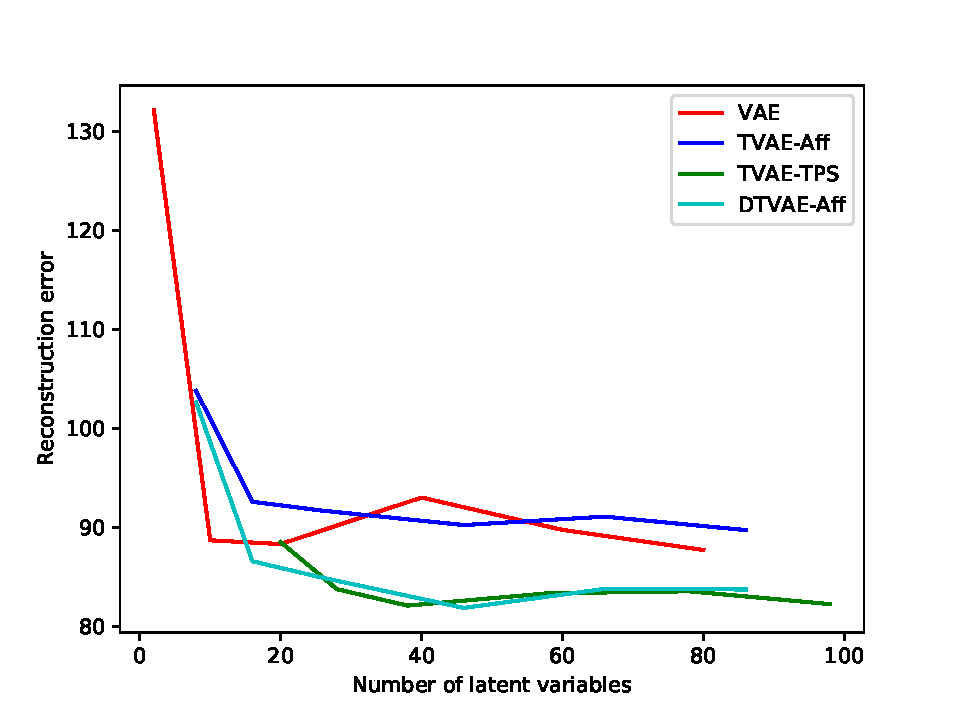
\includegraphics[scale=0.6]{num_latent.pdf}
\caption{-FINISH EXP FOR TVAE AND DTVAE-. Lower bound of the loglikelihood as a function of the dimensionality of the latent codes for the standard Variational Autoencoder (Normal priors and approximate posterior, Bernoulli conditional) and derived transformer models -TVAE, DTVAE- (with deterministic relation between x and the pose $u$). For each data point, the architecture of the network has been finetuned to optimize the loss.}
\label{numlatent}
\end{figure}

But this lower bound only gives information about the quality of the reconstruction and the scale of the latent variables. What is important for us is whether or not this model can produce credible samples. Before trying to derive objective measures for this, we generate samples from the three different models. Here, the focus is put on generating a new code $z$ and generating $x$ from $z$ (thanks to the decoder part of the network) and the average transformation observed on the training set for $u$. This means that we are not sampling the pose of the digit. We will discuss how to do that in a meaningful manner later. That is why, except for the VAE, all the samples are aligned in an upright direction.\\

\begin{figure}[H]
\centering
\begin{minipage}{.33\textwidth}
\begin{flushleft}
\begin{tabular}{|@{}c@{}|}
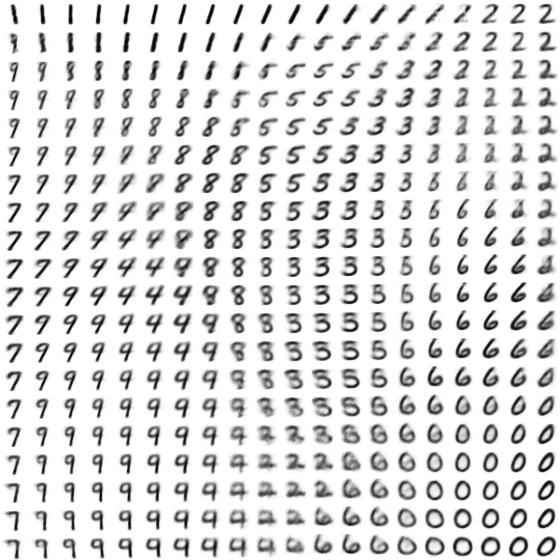
\includegraphics[scale=0.5]{manifold_18.jpg}\\ \hline
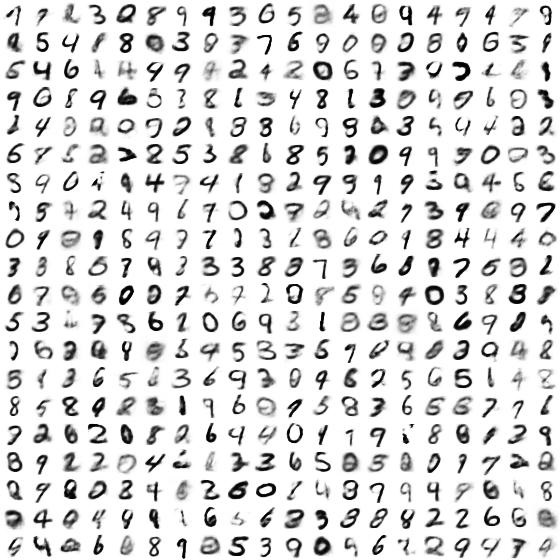
\includegraphics[scale=0.5]{manifold_19.jpg}\\ \hline
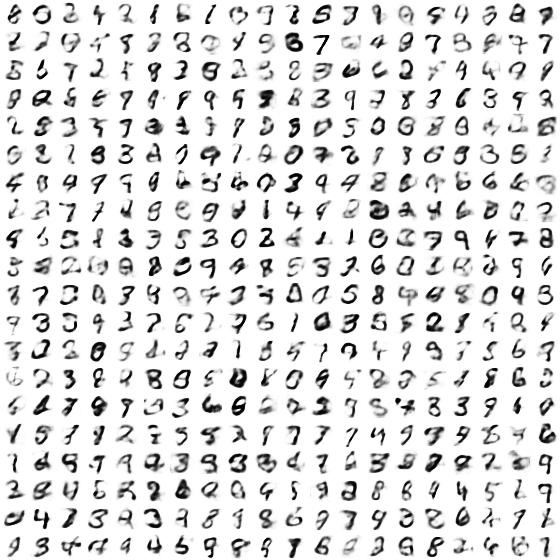
\includegraphics[scale=0.5]{manifold_20.jpg}\\
\end{tabular}
\end{flushleft}
\end{minipage}%
\begin{minipage}{.33\textwidth}
\begin{tabular}{|@{}c@{}|}
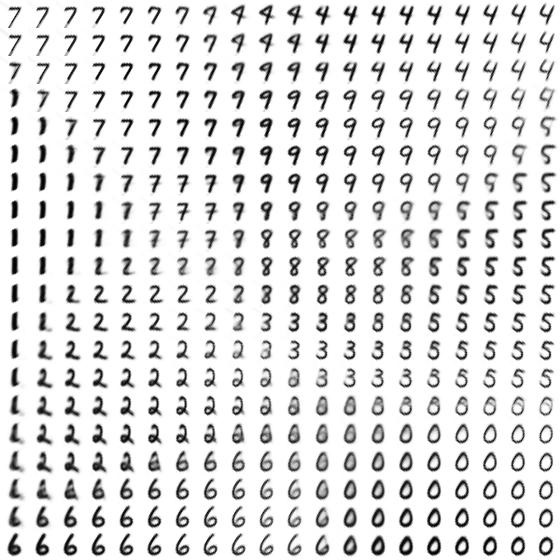
\includegraphics[scale=0.5]{manifold_26.jpg}\\ \hline
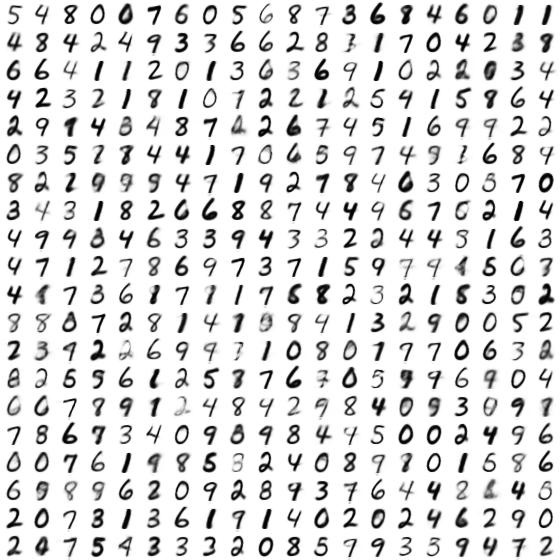
\includegraphics[scale=0.5]{manifold_27.jpg}\\ \hline
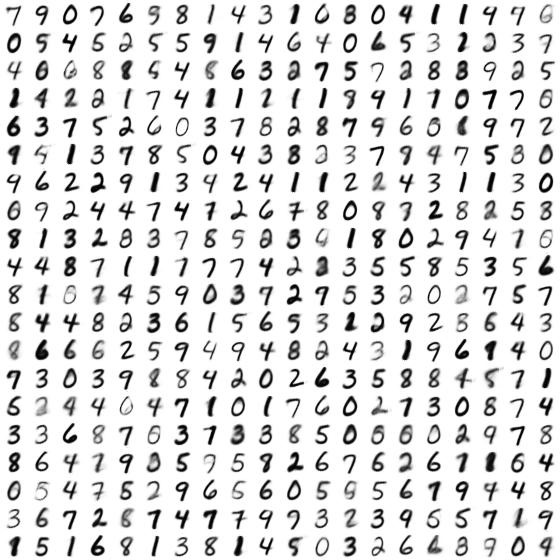
\includegraphics[scale=0.5]{manifold_28.jpg}\\
\end{tabular}
\end{minipage}%
\begin{minipage}{.33\textwidth}
\begin{tabular}{|@{}c@{}|}
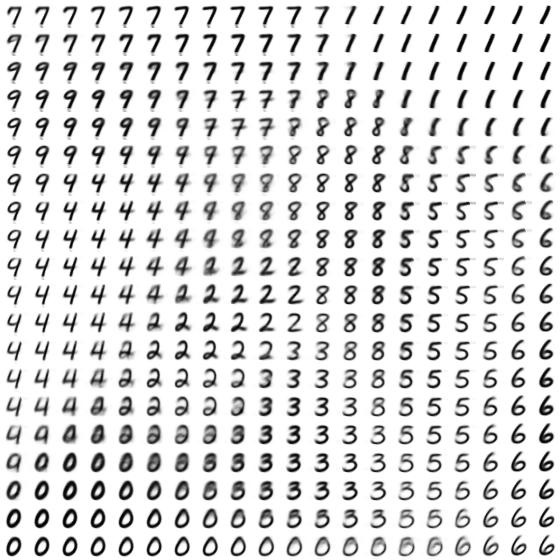
\includegraphics[scale=0.5]{manifold_32.jpg}\\ \hline
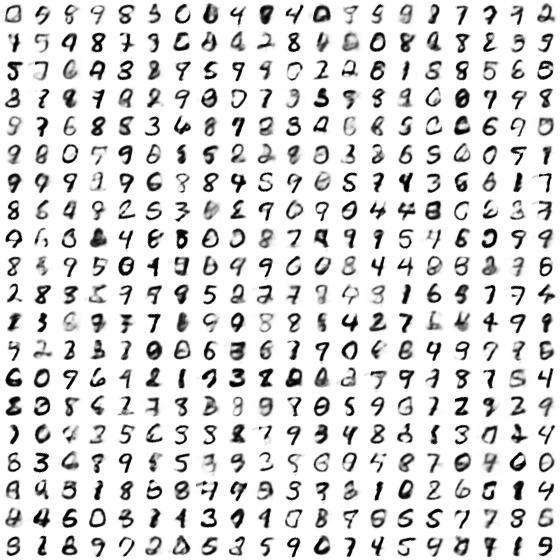
\includegraphics[scale=0.5]{manifold_33.jpg}\\ \hline
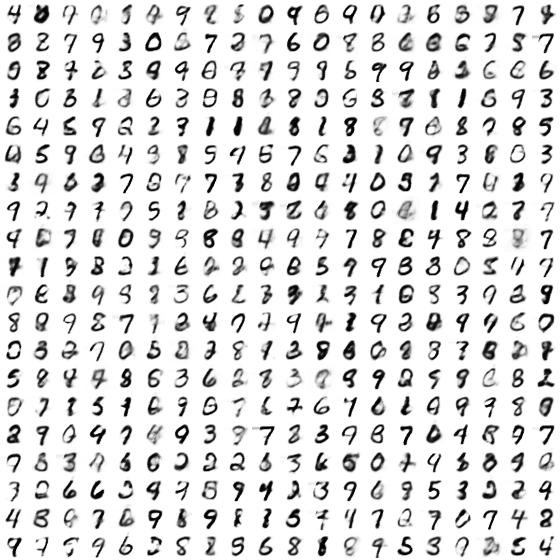
\includegraphics[scale=0.5]{manifold_34.jpg}\\
\end{tabular}
\end{minipage}

\caption{New samples generated by the models.Left: VAE. Middle: TVAE-Aff. Right: DTVAE-Aff. From top to bottom: respectively 2, 14, 24 dimensions for the latent code $z$.\\ For the first line, since the dimension is 2, $z$ varies continously on the 2D plane. For other lines, each cell is drawn independently from the corresponding multivariate standard normal.}
\label{generatedcomparison}
\end{figure}

\subsubsection{Discussion}

From figure \ref{generatedcomparison}, we can witness the previously mentioned drawbacks of the VAE: the bluriness on generated samples, as well as the decaying quality of samples when the number of latent variables grows. This shows in particular that a high likelihood does not imply nice generated images. As mentioned, the samples are in the upright direction for models which have a transformer layer, which means that the spatial regression part of each network is indeed working (as demonstrated in \cite{Siyu:vae}). We would like to point out the quality of the sample produced by the TVAE (middle column), which are sharp and whose quality does not seem to be affected by the number of latent variables. In an attempt to uncouple spatial information from the rest of the variability in the image, we designed the DTVAE. It performs poorly in terms of generating performances, and exhibits similar behavior to the VAE.\\

This helps us develop an intuition about why the TVAE produces such sharp samples. On the contrary to the DTVAE, the TVAE learns to regress an image on its upright version ($x$ on $y'$). This means that the part of the encoder which is not regressing the spatial parameters is in charge of suppressing the pose, and learns spatial invariance. Our interpretation is that it acts like an inner data augmentation, which gives a natural way to the network to regularize itself. As we will discuss in the "Further developments" section, it could mean that enhancing this part of the network with layers designed to better achieve spatial invariance could lead to a great improvement.\\
By using the TVAE, without using a prior on the pose $u$. We showed that we can fulfill all the properties of a classic autoencoder, while being able to generate new upright samples of good quality.

\subsection{Latent code information}
By the fixed machinery that we deployed, we know what the spatial variable $u$ contains, but did this reparametrization of the problem help disentangle the information in $z$? --> Add study on varying one component of $z$ at a time.


\subsection{Distribution over the latent spatial variables}

Since the TVAE shows nice properties, we will focus on it for the rest of the paper. As the transformer layer \cite{Jaderberg.stn} permits, we can use affine transformations as well as thin plate splines to model the deformations in the image. We can see from figure \ref{generatedafftps} that at least visually, the TPS seems to offer slightly sharper samples on average.\\

\begin{figure}[h]
\centering
\begin{minipage}{.33\textwidth}
\begin{tabular}{|@{}c@{}|}
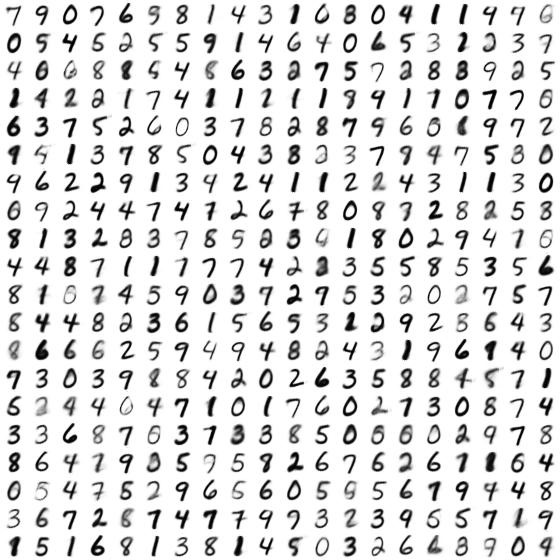
\includegraphics[scale=0.5]{manifold_28.jpg}\\
\end{tabular}
\end{minipage}%
\begin{minipage}{.33\textwidth}
\begin{tabular}{|@{}c@{}|}
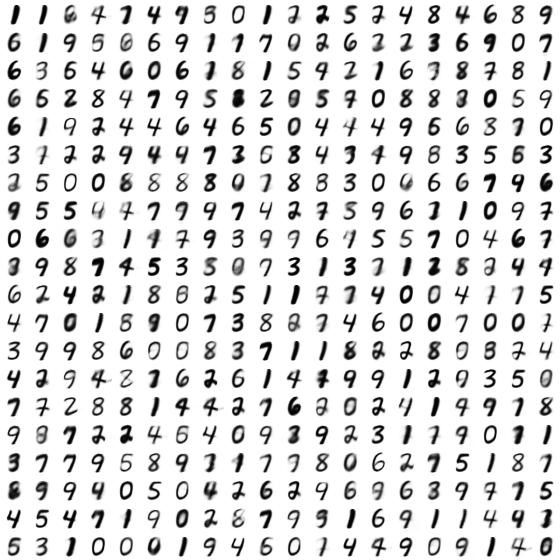
\includegraphics[scale=0.5]{manifold_39.jpg}\\
\end{tabular}
\end{minipage}%
\caption{New samples generated by the models.Left: TVAE with affine transformer. Right: TVAE with thin plate splines transformer. We use 30 dimensions for the latent code (left: $dim(z) = 24$, $dim(u) = 6$; right: $dim(z) = 12$, $dim(u) = 18$) .Each cell is drawn independently from the corresponding multivariate standard normal.}
\label{generatedafftps}
\end{figure}

There is a few things to consider before putting sensible priors on those quantities. First, they have a physical meaning, and act directly on the image through the transformer, on the contrary to z. This means in particular that we cannot simply put a normal prior with mean 0 and variance 1, because that would mean that the average transformation is the identity and that the variability is arbitrary. For the latent code $z$, it did not matter because the neural network itself can take care of setting the scale to a sensible value. This means that we have to estimate some parameters of the prior during the optimisation process. Secondly, we have to pay attention to the covariance structure of $u$. If we look at the approximate posterior distribution of $u$, there is correlations between components (up to 30\% for the affine mapping). This is actually quite natural; for the affine correlations, the matrix with 6 cells has actually an inner structure in terms of rotation $\psi$, shearing $(S_x, S_y)$, and translation $(T_x, T_y)$:\\

$M=
  \left[ {\begin{array}{ccc}
   a & b & c\\
   d & e & f\\
  \end{array} } \right]
 = 
  \left[ {\begin{array}{ccc}
   S_x cos \psi & -S_x sin \psi & S_x T_x\\
   S_y sin \psi & S_y cos \psi & S_y T_y\\
  \end{array} } \right]$

  Therefore, it might be better to put priors on those 5 interpretable variables than on the 6 cells of the matrix. A sensible prior in this case could be:\\
  $u = (\psi, log S_x, log S_y, T_x, T_y) \sim N(\nu^u, Diag(\tau_1^u, \tau_2^u, \tau_3^u, \tau_4^u, \tau_5^u))$

  The same problem arise for the thin plate splines. The 9 points of the grid we have been using previously share a lot of dependence. In the case of a rotation centered in the middle of the grid, all exterior points move together and are coupled in a non linear fashion. This implies that using a gaussian prior (even with a dense covariance matrix) may fail to model the range of transformations.\\

  In figure \ref{generatedwithpose}, we made a comparison of different priors on the affine and TPS version of the TVAE. The first conclusion we can draw is that centering the prior on the identity mapping yields poor results. There is coadaptation between the values of $z$ and $u$, and the procedure seems to find a local optima by internally representing the digit slighlty zoomed in and sheared to fit almost all the space available. We don't have any intuition about this phenomenon yet. But because the expected posterior transformation is far from being the identity, the procedure overestimated the prior variance, leading the samples with the sampled pose to be not satisfactory. If the mean is fitted, a gaussian prior on the 6 degrees of freedom of the affine transformation yield digits that are mainly sheared in the horizontal direction.\\

    Using the suggested prior on the reparametrized transformation with 5 degrees of freedom introduce a noticeable variation in rotation. We could argue that some numbers do not seem to be in a "natural" pose. Our interpretation is that even if we assumed that the pose(contained in $u$) and the class (contained in $z$) of the sample were independent, there is probably still dependence between the two. A visual way to understand this lies in figure \ref{generatedcomparison}. The long bar shared by the 7, the 1 and the 9 all have the same orientation. But the 1 is usually vertical in the dataset. This means that there is once again a coadaptation between the general-purpose latent code $z$ and the pose $u$.

\begin{figure}[h]
\centering
\begin{minipage}{.5\textwidth}
\centering
\begin{tabular}{|@{}c@{}|}
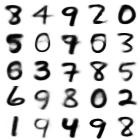
\includegraphics[scale=1]{manifold_ident_50.jpg}\\ \hline
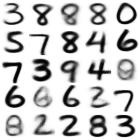
\includegraphics[scale=1]{manifold_ident_51.jpg}\\ \hline
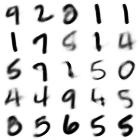
\includegraphics[scale=1]{manifold_ident_52.jpg}\\
\end{tabular}
\end{minipage}%
\begin{minipage}{.5\textwidth}
\centering
\begin{tabular}{|@{}c@{}|}
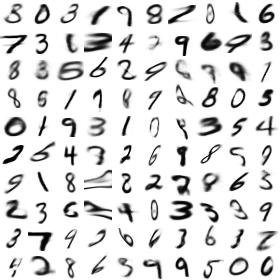
\includegraphics[scale=1]{manifold_sig_50.jpg}\\ \hline
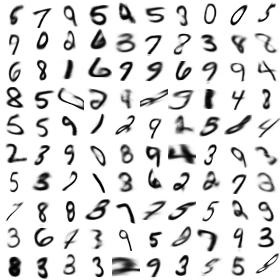
\includegraphics[scale=1]{manifold_sig_51.jpg}\\ \hline
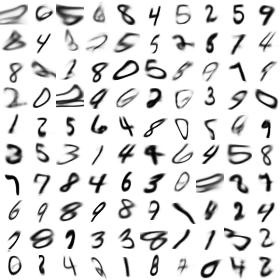
\includegraphics[scale=1]{manifold_sig_52.jpg}\\
\end{tabular}
\end{minipage}%
\caption{Left: samples generated by a draw from the prior of the general latent code $z$. Right: same samples transformed by a draw from the distribution on of the spatial latent variable $u$. From top to bottom, different priors: normal prior with mean fixed to identity, fitted diagonal covariance on affine transformation with 6 d.o.f; normal prior with fitted mean, fitted diagonal covariance on affine transformation with 6 d.o.f; normal prior with fitted mean, fitted diagonal covariance on reparametrized affine transformation with 5 d.o.f. ; --to be added TPS transformation, fitted mean, fitted diagonal covariace, 18 dof.}
\label{generatedwithpose}
\end{figure}

\section{Future Work}

- to do: CNN - TVAE for Mnist
- propose architecture on CIFAR10

\section{Conclusion}
[placeholder]
%----------------------------------------------------------------------------------------
%   REFERENCE LIST
%----------------------------------------------------------------------------------------
\bibliographystyle{unsrt}
\bibliography{biblio}


\end{document}